%%%%%%%%%%%%%%%%%%%%%%%%%%%%%%%%%%%%%%%%%%%%%%%%%%%%%%%%%%%%%%%%%%
\section{DEN2NE}
\label{sec:den2ne}

\acrfull{den2ne}\footnote{https://github.com/NETSERV-UAH/den2ne-Alg} \cite{den2ne} \cite{gitden2ne} se presenta como un algoritmo diseñado por el equipo de investigación NetIS de la \gls{uah} para la automatización del proceso de encaminamiento y de compartición de recursos de forma eficiente. Su aplicación en este \gls{tfm} se enfoca en el ámbito de las \gls{sg}s para llevar a cabo el proceso de distribución energética entre los diferentes prosumidores (ver Sección \ref{sec:prosu}) que participan en la red. No obstante, \gls{den2ne} está diseñado para emplearse en cualquier entorno distribuido donde los nodos necesiten colaborar, compartir e intercambiar recursos para lograr objetivos comunes.

\vspace{3mm} 

El algoritmo se enfoca en la búsqueda de nodos vecinos para llevar a cabo la distribución energética. En este proceso de intercambio de recursos se asumen conexiones bidireccionales entre los nodos para representar la oferta y la demanda existente. Es preciso indicar que \gls{den2ne} se fundamenta en los siguientes principios: escalabilidad, versatilidad, flexibilidad y resiliencia. En el caso de la escalabilidad, el algoritmo minimiza los tiempos de convergencia para posibilitar la aplicación del mismo en topologías densas, tomando importancia del consumo de recursos de memoria y minimizando el número de mensajes transmitidos. 

\vspace{3mm}

En cuanto a la resiliencia, se obtienen rutas de espaldo de cada prosumidor a un nodo raíz o \textit{gateway}, que, en el caso de uso de las \gls{sg}s, daría acceso a la red de distribución eléctrica y se asumiría que está conectado a recursos infinitos. Este nodo toma la responsabilidad de funcionar como balanceador, puesto que el principal objetivo de \gls{den2ne} viene dado por la compensación de los recursos de la red a nivel global. A modo de visualizar de una forma gráfica este proceso, se muestra en la Figura \ref{fig:balance} un ejemplo de una red compuesta por seis nodos y un \textit{gateway}. Como se puede apreciar, se representa tanto la conectividad que existe entre los nodos (color negro), como el sentido del intercambio de los recursos hacia el \textit{gateway} (color naranja). 

\vspace{3mm}

\begin{figure}[H]
  \centering
  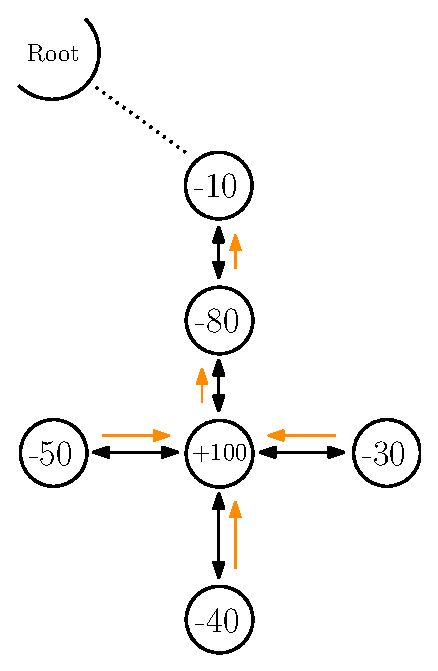
\includegraphics[width=0.4\textwidth]{img/teoria/fig2.eps}
  \caption{Ejemplo del proceso de balance de recursos \cite{den2ne}}
  \label{fig:balance}
\end{figure}

\vspace{3mm}

Teniendo esto en cuenta, el primer paso que lleva a cabo \gls{den2ne} se basa en una asignación jerárquica de etiquetas. Mediante este proceso, cada nodo obtendrá uno o varios identificadores numéricos (IDs), a partir de los que podrá definir su posición relativa en la topología respecto al nodo raíz. Al aplicar este paso, se calculan todos los caminos que existen desde cada nodo hacia el \textit{gateway} y se tratan los posibles bucles que puedan producirse al asignar las etiquetas como se representa en la Figura \ref{fig:bucle}.

\vspace{3mm}

\begin{figure}[h!]
  \centering
  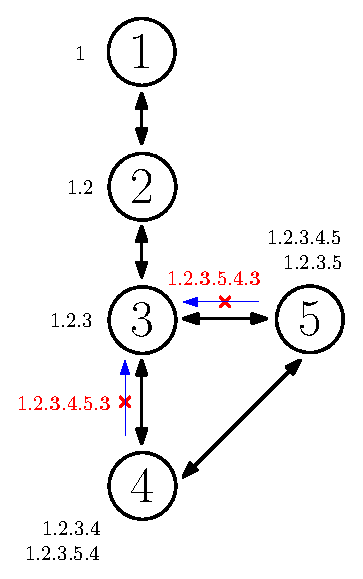
\includegraphics[width=0.35\textwidth]{img/teoria/fig4.eps}
  \caption{Proceso de asignación de etiquetas \cite{den2ne}}
  \label{fig:bucle}
\end{figure}

\vspace{3mm}

En el caso de que \gls{den2ne} sea configurado para asignar varias etiquetas a cada nodo, se añade un paso de selección, en el que se escogerá una única etiqueta de las asignadas anteriormente. Es decir, para cada nodo se comprobará qué identificador (ID) es el más apropiado y se activará, tomando en consideración alguno de los seis criterios establecidos por el algoritmo. Estos criterios vienen determinados por el número de saltos o distancia (física o lógica) al nodo raíz, las pérdidas de enlace, el balance de potencia o las combinaciones de algunos de los anteriores. Con el proceso de selección, se establecerá la topología lógica y, por tanto, los caminos finales desde cada nodo al \textit{gateway}. No obstante, las etiquetas no seleccionadas pueden ser útiles ante la necesidad de caminos opcionales, en el caso de que alguno de los nodos falle.

\vspace{3mm}

Como se introducía al comienzo de la presente Sección, el objetivo del algoritmo es alcanzar una situación final de balance global energético en la red. Para que este proceso sea eficiente, se debe seguir un orden de distribución basado en la longitud del identificador que caracteriza a cada nodo. \gls{den2ne}, al ser centralizado, puede recolectar la lista de etiquetas de la topología completa y comenzar el proceso por los nodos más lejanos al \textit{gateway}. 

\vspace{3mm}

Por consiguiente, cada uno de los nodos existentes redireccionará el propio exceso de demanda u oferta de energía hacia su nodo padre, repitiéndose el procedimiento hasta llegar al nodo raíz. De forma concluyente, se puede apreciar en la Figura \ref{fig:distri} cómo se definirá un escenario de red en el que todos los nodos tendrán un valor energético nulo, a excepción del nodo raíz, que acumulará el valor total de todos los intercambios producidos en la red. Cabe destacar que en el proceso de distribución energética es configurable el tipo de escenario, que puede ser ideal, con pérdidas, con capacidad de enlace limitada o con pérdidas y capacidad de enlace limitada. De la misma forma, el algoritmo establece para cada nodo los recursos energéticos iniciales, siguiendo una función de densidad de probabilidad.

\vspace{3mm}

\begin{figure}[h!]
  \centering
  \begin{minipage}{0.5\textwidth}
    \centering
    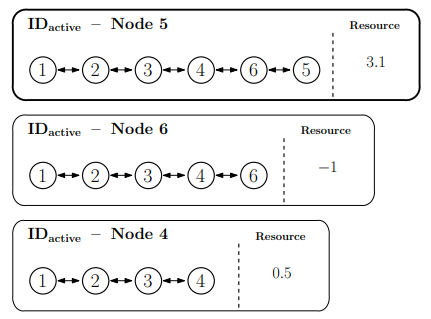
\includegraphics[width=\linewidth]{img/teoria/distri1.png}
    \label{fig:distri1}
  \end{minipage}\hfill
  \begin{minipage}{0.5\textwidth}
    \centering
    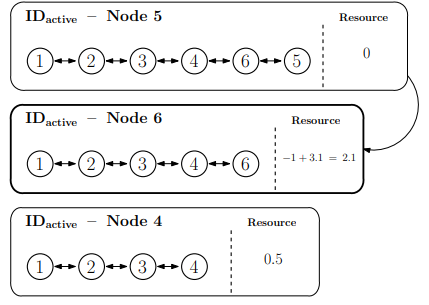
\includegraphics[width=\linewidth]{img/teoria/distri2.png}
    \label{fig:distri2}
  \end{minipage}\hfill
  \begin{minipage}{0.5\textwidth}
    \centering
    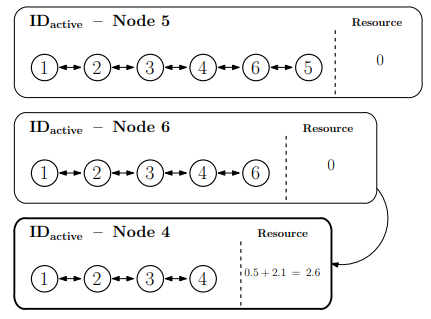
\includegraphics[width=\linewidth]{img/teoria/distri3.png}
    \label{fig:distri3}
  \end{minipage}
  \caption{Proceso de distribución energética \cite{den2ne}}
  \label{fig:distri}
\end{figure}

